\section{Aquisição}

\begin{frame}{Aquisição}

    Processo que combina os scans do laser e as imagens da câmara para produzir uma nuvem de pontos colorizada.

\end{frame}

\begin{frame}{Acquisição}

    Para produzir o set de imagens e laserscans, o pan-tilt é movimentado numa interpolação num espaço de ângulos.

    Existem uma lista de waypoints para a obtenção das imagens.

    Os laserscans são obtidos no movimento entre os waypoints.

\end{frame}

\begin{frame}{Pipeline}
    
    Dois processos sequenciais:

    \begin{enumerate}
        \item \textbf{Transformação} e \textbf{acumulação} dos Laserscans em uma nuvem de pontos não colorizada.
        \item \textbf{Registo} das imagens na nuvem de pontos.
    \end{enumerate}

\end{frame}

\begin{frame}{Transformação e Acumulação}
        
    \begin{enumerate}
        \item<1-> Transformação dos Laserscans em nuvens de pontos no referencial do laser.
        \item<2-> Transformação das nuvens de pontos no referencial estático do robot (\textit{base\_link}).
        \item<3-> Acumulação dos pontos numa nuvem de acumulação.
    \end{enumerate}

\end{frame}


\begin{frame}[fragile]{Registo de cor}

    \begin{verbatim}
for image := images
    for point := pointCloud
        pointInCamera := transform(point, baseToCameraTF)
        u,v := project3dToUV(pointInCamera, cameraK)
        if (u,v) > (0,0) and (u,v) < (width, height)
            color := image[u, v]
        end
    end
end
    \end{verbatim}

\end{frame}

\begin{frame}{Registo de cor}

    \begin{enumerate}
        \item Para cada imagem existe um registo, ou seja, uma nuvem de pontos colorizada parcial.
        \item A nuvem de pontos final é uma acumulação das nuvens parciais, através de uma heurística (por exemplo, Last One Wins).
    \end{enumerate}
    
\end{frame}

\begin{frame}{Problemas}

    \begin{itemize}
        \item Qualidade geométrica e de registo é dependente de uma boa calibração.
        \item Várias cores para o mesmo pixel. Como selecionar a cor certa?
        \item Cor pode não ser uniforme durante a aquisição, o que implica que superfícies de cor uniforme não aparecem uniformes (exposição, sensibilidade, iluminação).
        \item Existe muita oclusão, mas pode ser obtida pela fusão de várias aquisições.
    \end{itemize}

\end{frame}

\begin{frame}{Problemas Geométricos}

    \begin{figure}
        \centering
        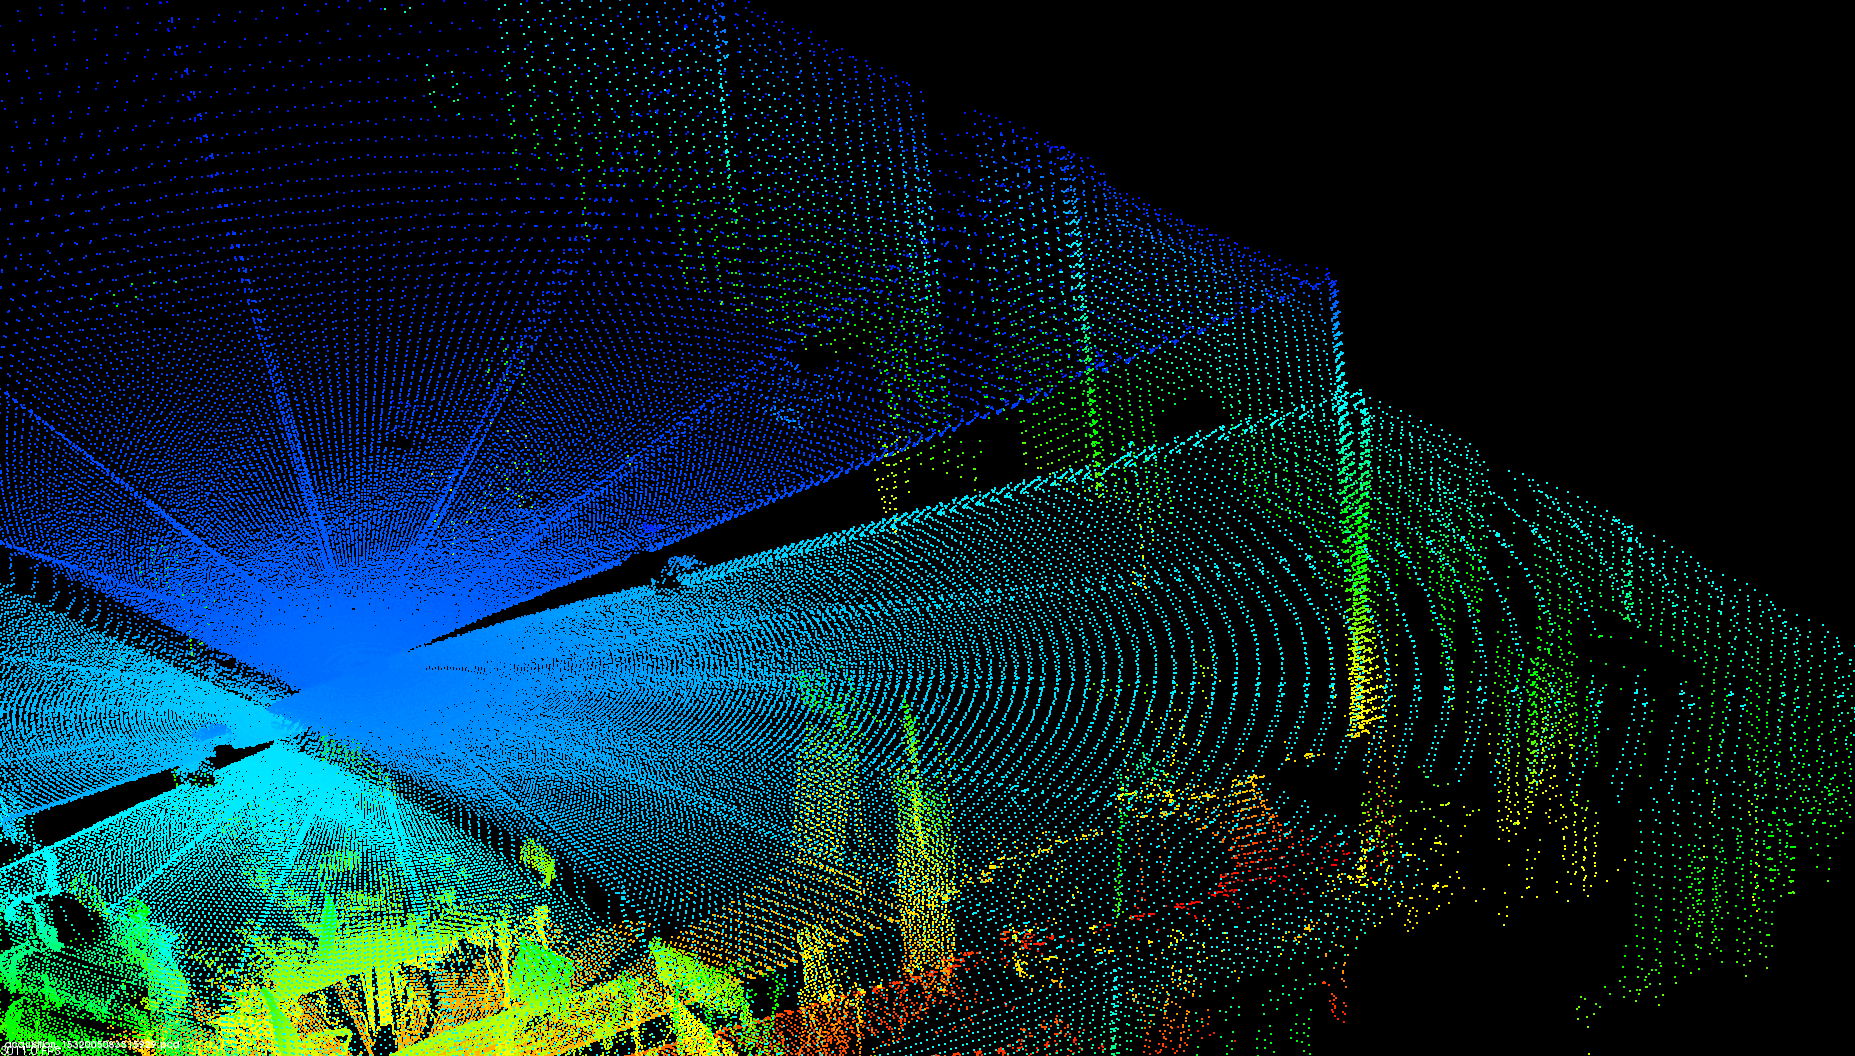
\includegraphics[width=1\textwidth]{img/geometric_errors_1.png}
    \end{figure}
    
\end{frame}

\begin{frame}{Problemas Geométricos}

    \begin{figure}
        \centering
        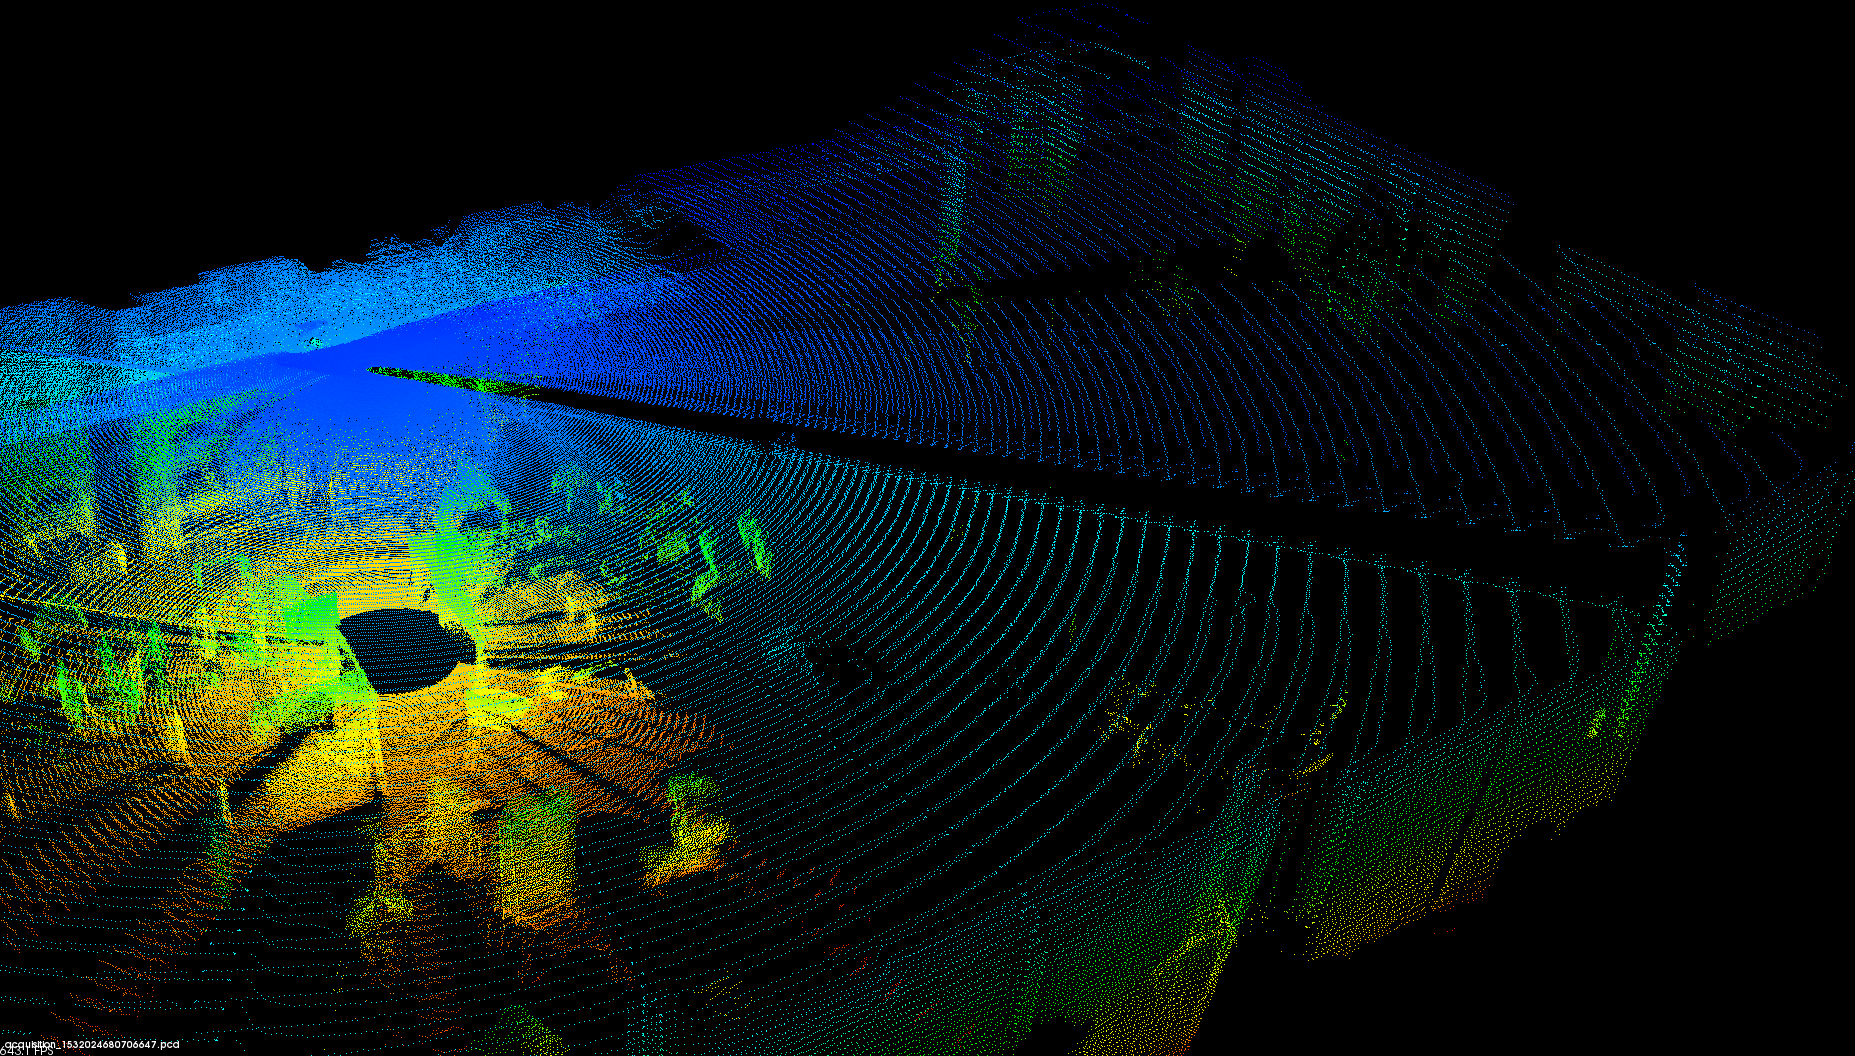
\includegraphics[width=1\textwidth]{img/geometric_errors_2.png}
    \end{figure}
    
\end{frame}

\begin{frame}{Problemas Cor}

    \begin{figure}
        \centering
        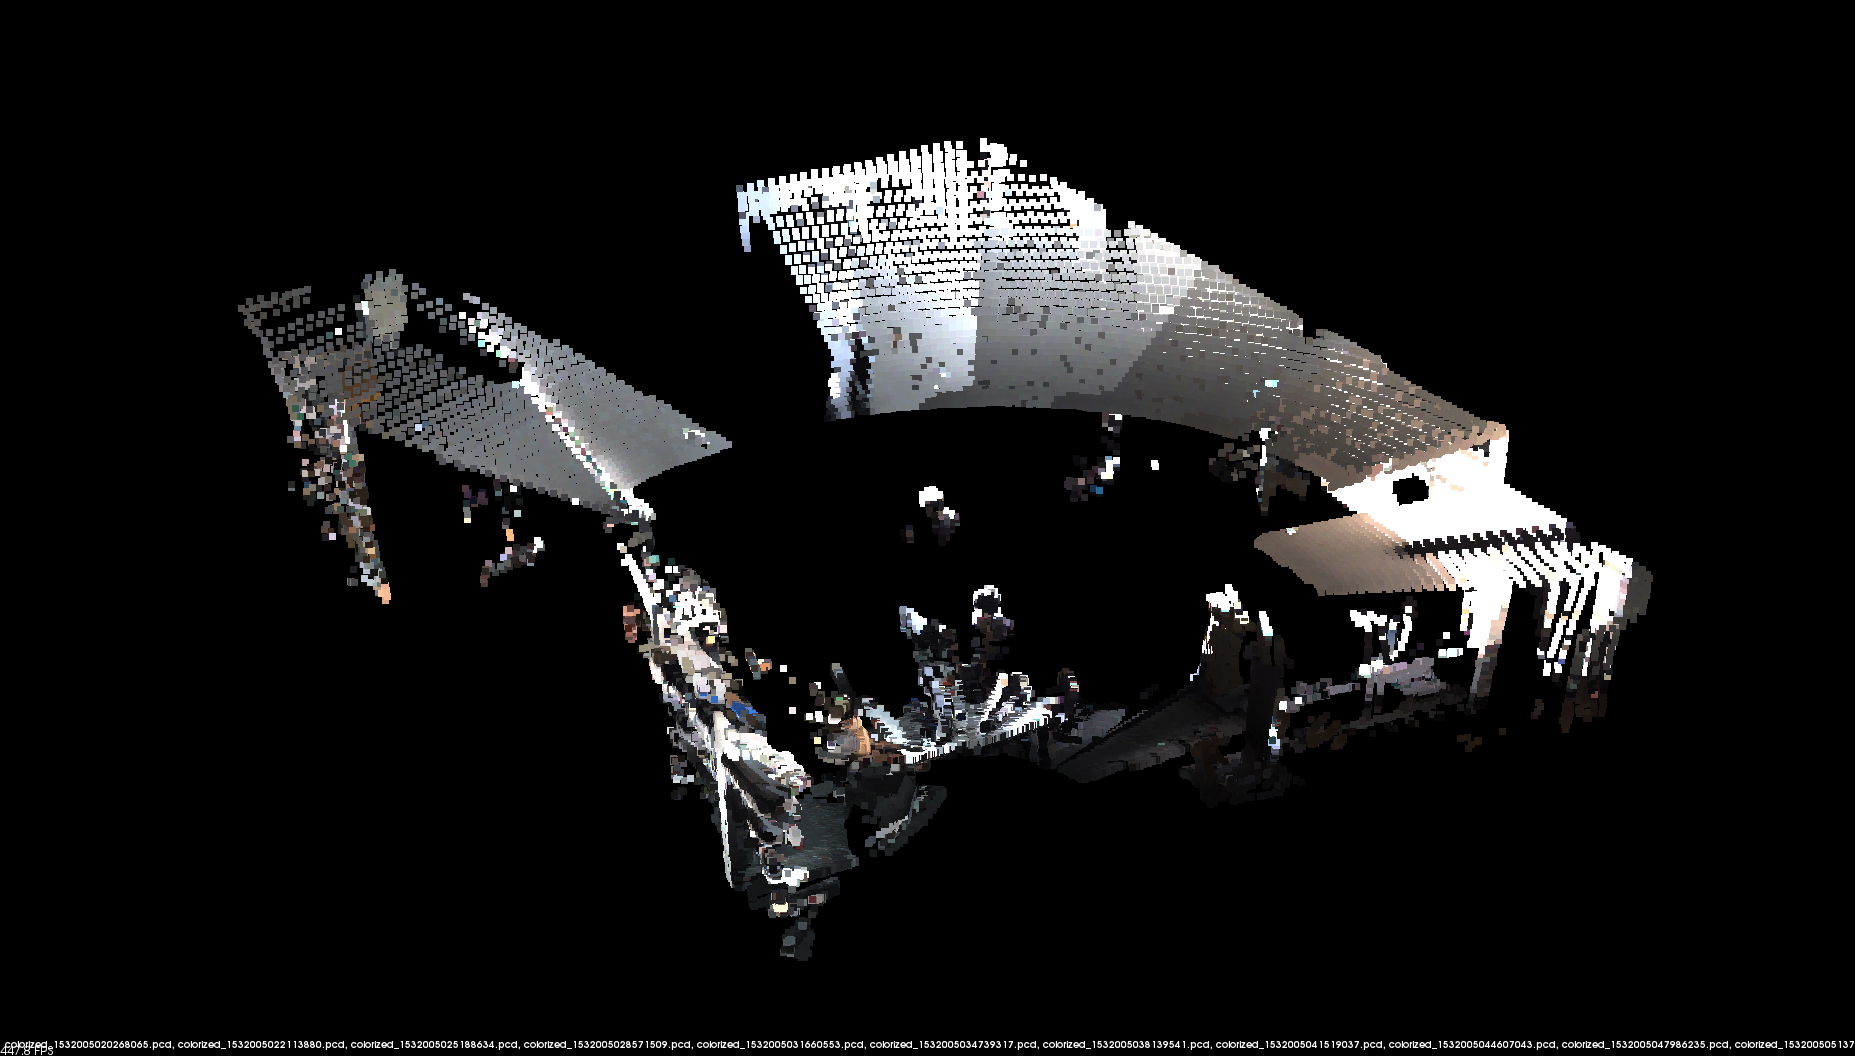
\includegraphics[width=1\textwidth]{img/color_errors_1.png}
    \end{figure}
    
\end{frame}

\begin{frame}{Problemas Cor}

    \begin{figure}
        \centering
        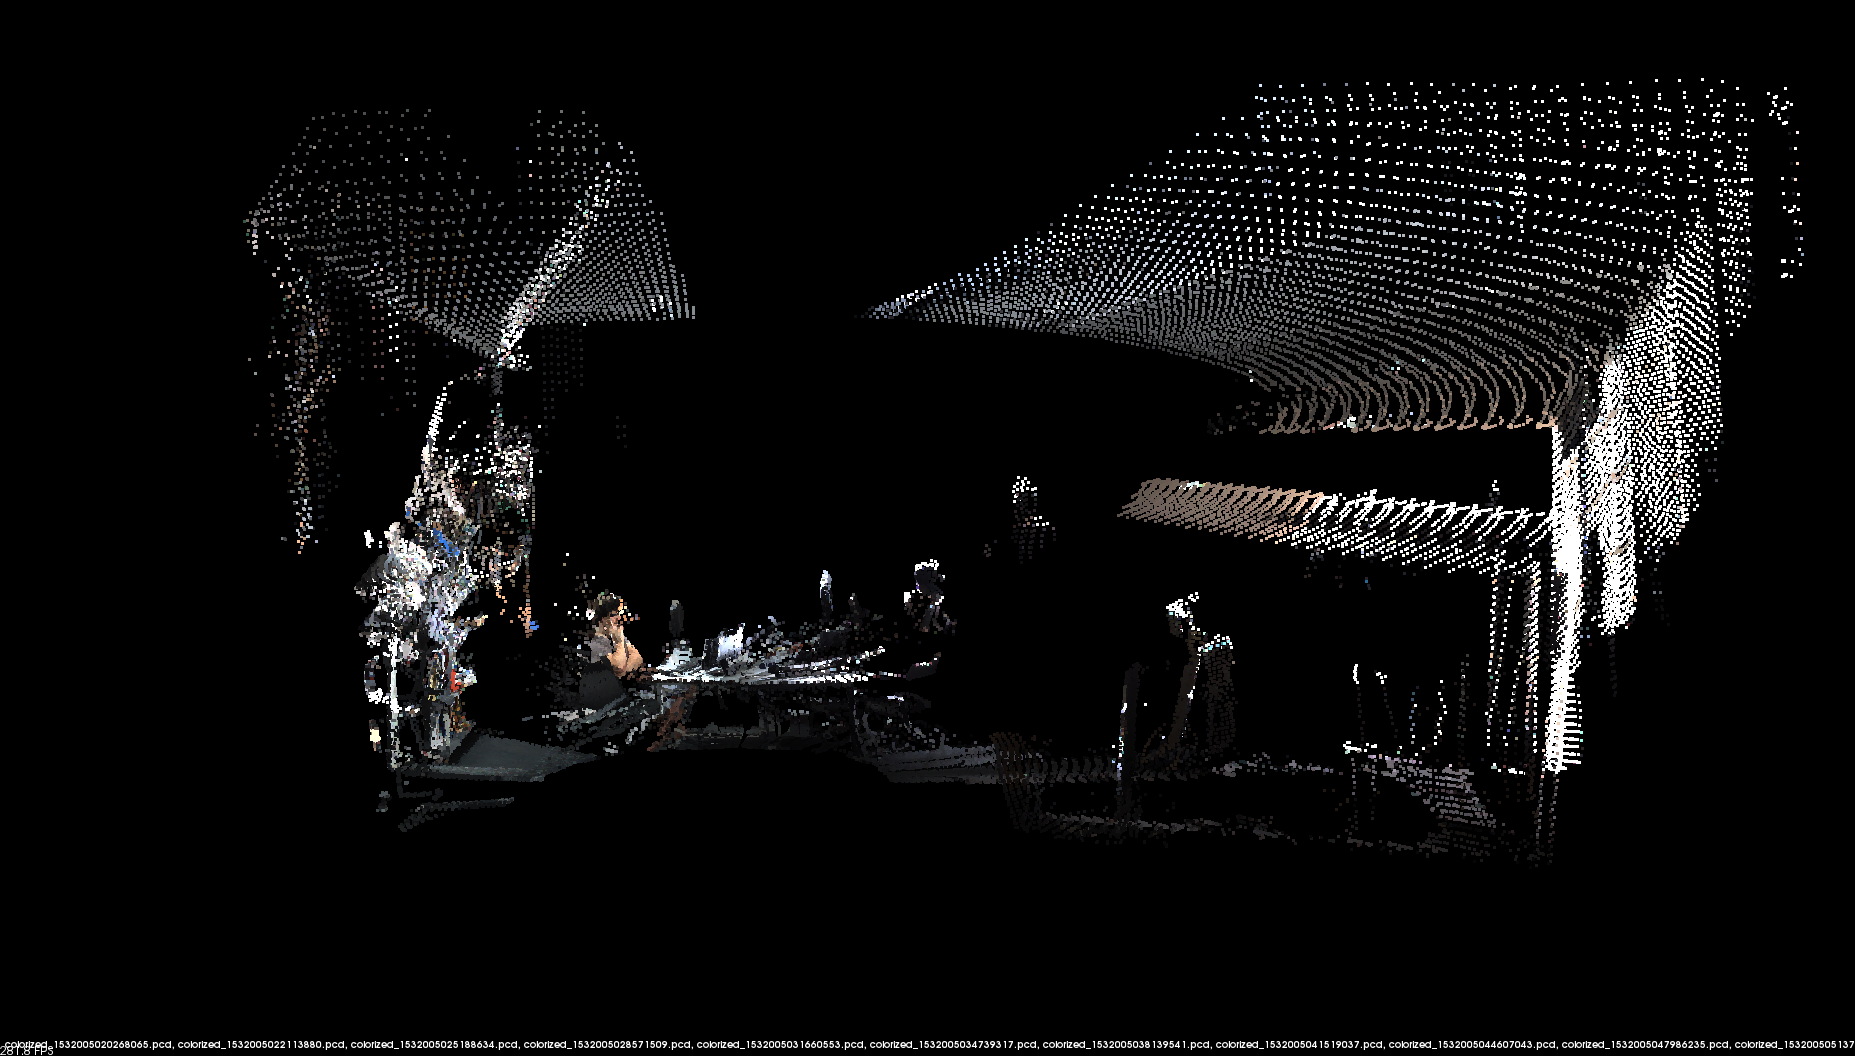
\includegraphics[width=1\textwidth]{img/color_errors_2.png}
    \end{figure}
    
\end{frame}

\begin{frame}{Problemas Registo}

    \begin{figure}
        \centering
        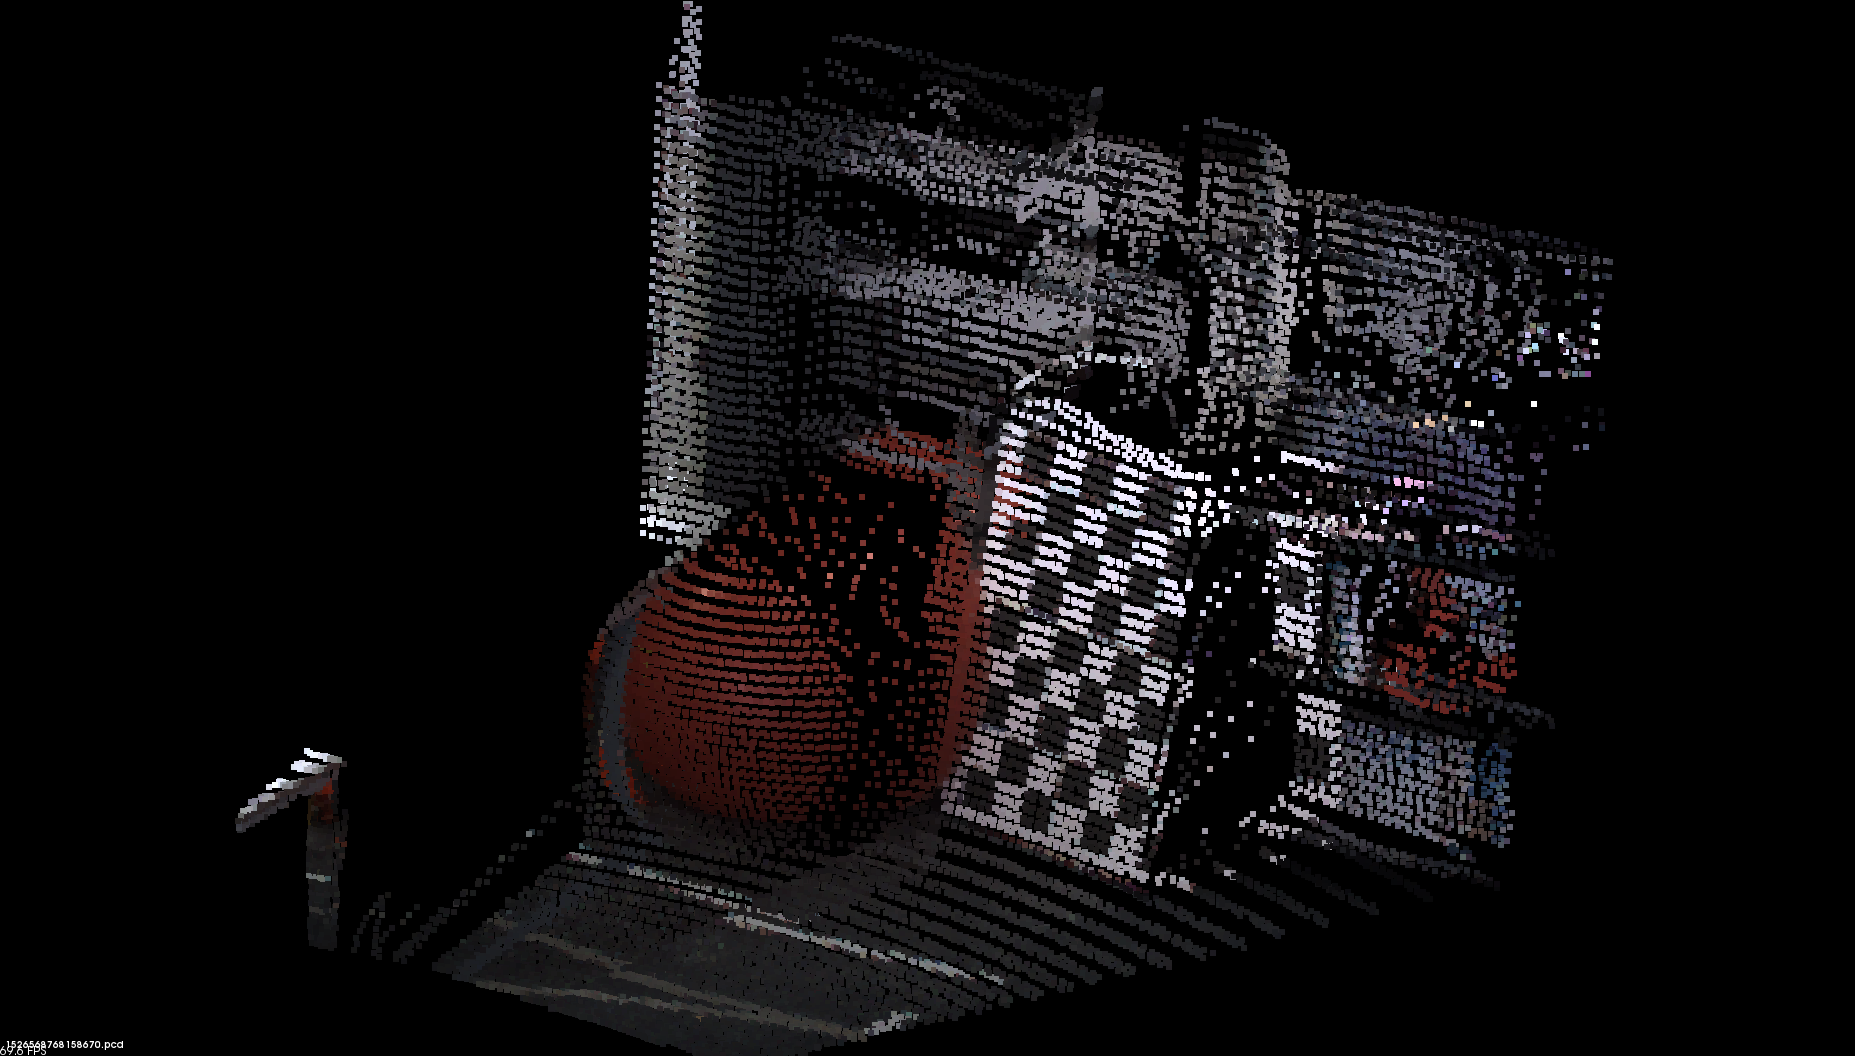
\includegraphics[width=1\textwidth]{img/radlocc_bad_regist.png}
    \end{figure}
    
\end{frame}